\newpage % saltar a la siguiente pagina

\section{Dibujando formas con canvas}

Ahora que hemos preparado nuestro entorno \code{canvas}, podemos entrar en detalles de cómo dibujar en el \code{canvas}. Al final de esta sección, habrás aprendido cómo dibujar rectángulos, triángulos, líneas, arcos y curvas, familiarizándote con algunas de las formas básicas. Trabajar con trazados es esencial a la hora de dibujar objetos en el \code{canvas} y veremos cómo hacerlo.

\subsection{La cuadrícula}

Antes de empezar a dibujar, tenemos que hablar de la cuadrícula del \code{canvas} o del espacio de coordenadas. Nuestra estructura \texthtml{HTML} de la sección anterior tenía un elemento de \code{canvas} de 150 pixels de ancho y 150 pixels de alto.

\vspace{0.5cm} % separación vertical
\begin{center}
	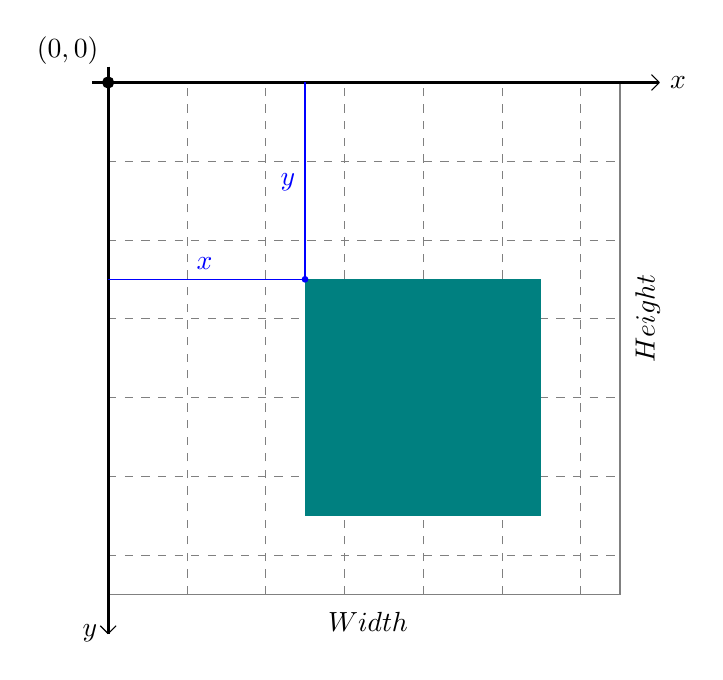
\begin{tikzpicture}
		\draw[color=gray, help lines, dashed] (0,0) grid (6.5,-6.5);
		\draw[color=gray] (0,0) rectangle (6.5,-6.5); % Cuadrado de esquina (0,0) a (2,2)
		\node[color=black, rotate=90, yshift=-10pt] at (6.5,-3) {$Height$};
		\node[color=black, yshift=-10pt] at (3.3,-6.5) {$Width$};

		% Ejes x e y
		\draw[color=black, very thick] (-0.2,0) -- (7,0) node[right] {$x$};
		\draw[color=black, very thick] (0,0.2) -- (0,-7) node[left] {$y$};

		% flechas
		\draw[color=black] (7,0) to (6.9, 0.1);
		\draw[color=black] (7,0) to (6.9, -0.1);
		\draw[color=black] (0, -7) to (0.1, -6.9);
		\draw[color=black] (0, -7) to (-0.1, -6.9);

		% Marcar el origen (0,0)
		\filldraw[color=black] (0,0) circle (2pt) node[anchor=north east, yshift=20pt] {$(0,0)$};

		% Flechas indicando la posición del punto (5, -5)
		\draw[color=blue] (2.5,0) -- (2.5,-2.5);
		\draw[color=blue] (0,-2.5) -- (2.5,-2.5);

		% Etiquetar los ejes de punto (2.5, -2.5)
		\node[color=blue, above right] at (1,-2.5) {$x$};
		\node[color=blue, above left] at (2.5,-1.5) {$y$};

		% Dibujar un cuadrado con color
		\fill[color=teal] (2.5, -2.5) rectangle (5.5, -5.5);
		\filldraw[color=blue] (2.5,-2.5) circle (1pt);

		% Marcar el punto (2.5, -2.5)
	\end{tikzpicture}
\end{center}
\vspace{0.5cm} % separación vertical


Normalmente, 1 unidad en la cuadrícula corresponde a 1 pixel en el canvas. El origen de esta cuadrícula se sitúa en la esquina superior izquierda en la \lineCode{coordenada (0,0)}. Todos los elementos se colocan en relación con este origen. Así que la posición de la esquina superior izquierda del cuadrado azul se sitúa a \code{X} pixels de la izquierda y a \code{Y} pixels de la parte superior, en la coordenada \code{(x,y)}. Más adelante en esta sección veremos cómo podemos trasladar el origen a una posición diferente, rotar la cuadrícula e incluso escalarla, pero por ahora nos ceñiremos a la posición por defecto.

\subsection{Dibujar rectángulos}

A diferencia de \textblue{SVG}, \taghtml{\textless canvas\textgreater} sólo admite dos formas primitivas: rectángulos y trazados (listas de puntos conectados por líneas). Todas las demás formas deben crearse combinando uno o más trazados. Por suerte, tenemos un surtido de funciones de dibujo de trazados que hacen posible componer formas muy complejas.

Primero veamos el \code{rectángulo}. Hay tres funciones que dibujan rectángulos en el canvas:

\vspace{0.5cm} % separación vertical
\begin{lstlisting}[language=TypeScript, style=mystyle]
  // (1) Dibuja un rectangulo relleno.
  fillRect(x, y, width, height)
\end{lstlisting}

\newpage % saltar a la siguiente pagina


\begin{lstlisting}[language=TypeScript, style=mystyle]
  // (2) Dibuja un contorno rectangular.
  strokeRect(x, y, width, height) (en-US)
\end{lstlisting}

\begin{lstlisting}[language=TypeScript, style=mystyle]
  // (3) Borra el area rectangular especificada, haciendola totalmente transparente.
  clearRect(x, y, width, height)
\end{lstlisting}
\vspace{0.5cm} % separación vertical

Cada una de estas tres funciones toma los mismos parámetros. \textblue{x} y \textblue{y} especifican la posición en el \code{canvas} (relativa al origen) de la esquina superior izquierda del rectángulo. \code{width} y \code{height} proporcionan el tamaño del rectángulo.

A continuación se muestra la función \code{draw()} de la página anterior, pero ahora hace uso de estas tres funciones.

\subsubsection*{Ejemplo de forma rectangular:}

\begin{lstlisting}[language=TypeScript, style=mystyle]
  function draw() {
    const canvas = document.getElementById("canvas");
    if (canvas.getContext) {
      const ctx = canvas.getContext("2d");

      ctx.fillRect(25, 25, 100, 100);
      ctx.clearRect(45, 45, 60, 60);
      ctx.strokeRect(50, 50, 50, 50);
    }
  }
\end{lstlisting}
\vspace{0.5cm} % separación vertical

La salida de este ejemplo seria este:

\vspace{0.5cm} % separación vertical
\begin{center}
	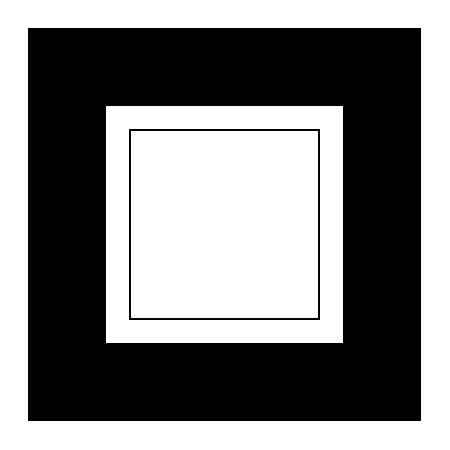
\begin{tikzpicture}
		\fill[black] (0, 0) rectangle (5, -5); % rectángulo negro
		\filldraw[white] (1, -1) rectangle (4, -4); % rectángulo blanco
		\draw[black] (1.3, -1.3) rectangle (3.7, -3.7); % rectángulo negro
	\end{tikzpicture}
\end{center}
\vspace{0.5cm} % separación vertical

La función \code{fillRect()} dibuja un gran cuadrado negro de 100 pixels en cada lado. La función \code{clearRect()} borra un cuadrado de 60x60 pixels del centro, y luego se llama a \code{strokeRect()} para crear un contorno rectangular de 50x50 pixels dentro del cuadrado borrado.

En las próximas páginas veremos dos métodos alternativos para \code{clearRect()}, y también veremos cómo cambiar el color y el estilo de trazo de las formas renderizadas.

A diferencia de las funciones de trazado que veremos en la siguiente sub-sección, las tres funciones de rectángulo dibujan inmediatamente en el canvas.

\newpage % saltar a la siguiente pagina
\subsection{Dibujando paths}

Veamos ahora los \code{paths}(trazos). Un \code{paths} es una lista de puntos, conectados por segmentos de líneas que pueden ser de diferentes formas, curvas o no; de diferente anchura y de diferente color. Un \code{path}, o incluso un sub-path, puede ser cerrado. Para hacer formas usando trazos, damos algunos pasos adicionales:

\begin{enumerate}
	\item Primero, se crea el path o trazo.
	\item Luego, se utiliza comandos de dibujo para dibujar en el path.
	\item Una vez creado el path, puedes trazar o rellenar el path para renderizarlo.
\end{enumerate}

\vspace{0.5cm} % separación vertical
Aquí están las funciones utilizadas para realizar estos pasos:

\begin{description}
	\listCustom{beginPath():} Crea un nuevo trazado. Una vez creado, los futuros comandos de dibujo se dirigen al trazado y se utilizan para construirlo.
	\listCustom{Métodos de path:} Métodos para establecer diferentes paths para los objetos.
	\listCustom{closePath():} Añade una línea recta al path, que va al inicio del sub-path actual.
	\listCustom{stroke():} Dibuja la forma trazando su contorno.
	\listCustom{fill():} Dibuja una forma sólida rellenando el área de contenido del trazo.
\end{description}

\vspace{0.5cm} % separación vertical
El primer paso para crear un trazo(\code{path}) es llamar a \code{beginPath()}. Internamente, los trazos se almacenan como una lista de sub-trazos (líneas, arcos, etc.) que juntos forman una forma. Cada vez que se llama a este método, la lista se restablece y podemos empezar a dibujar nuevas formas.

\vspace{0.5cm} % separación vertical
\begin{tcolorbox}
	[colback=red!5!white,colframe=cyan,fonttitle=\bfseries,title={\faLightbulbO\, Nota:}]

	Cuando el trazo actual está vacío, como por ejemplo inmediatamente después de llamar a \code{beginPath()}, o en un canvas recién creado, el primer comando de construcción del trazo siempre se trata como un \code{moveTo()}, independientemente de lo que realmente sea. Por esta razón, casi siempre querrá establecer específicamente su posición inicial después de reiniciar un trazo.
\end{tcolorbox}
\vspace{0.5cm} % separación vertical

El segundo paso es llamar a los métodos que realmente especifican los trazos a dibujar. Los veremos en breve.

El tercer paso, y opcional, es llamar a \code{closePath()}. Este método intenta cerrar la forma dibujando una línea recta desde el punto actual hasta el inicio. Si la forma ya ha sido cerrada o sólo hay un punto en la lista, esta función no hace nada.

\vspace{0.5cm} % separación vertical
\begin{tcolorbox}
	[colback=red!5!white,colframe=cyan,fonttitle=\bfseries,title={\faLightbulbO\, Nota:}]

	Cuando se llama a \code{fill()}, cualquier forma abierta se cierra automáticamente, por lo que no es necesario llamar a \code{closePath()}. Este no es el caso cuando se llama a \code{stroke()}.
\end{tcolorbox}
\vspace{0.5cm} % separación vertical

\newpage % saltar a la siguiente pagina
\subsubsection{Dibujar un triángulo}
Por ejemplo, el código para dibujar un triángulo sería algo así:

\vspace{0.5cm} % separación vertical
\begin{lstlisting}[language=TypeScript, style=mystyle]
  function draw() {
    const canvas = document.getElementById("canvas");
    if (canvas.getContext) {
      const ctx = canvas.getContext("2d");

      ctx.beginPath();
      ctx.moveTo(75, 50);
      ctx.lineTo(100, 75);
      ctx.lineTo(100, 25);
      ctx.fill();
    }
  }
\end{lstlisting}
\vspace{0.5cm} % separación vertical

El resultado se ve así:

\begin{center}
	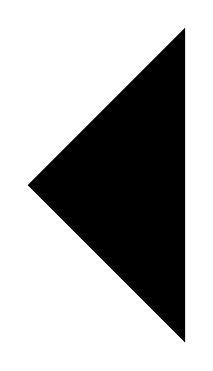
\begin{tikzpicture}
		\fill[black] (0,-2) -- (2,0) -- (2,-4) -- cycle;
	\end{tikzpicture}
\end{center}
\vspace{0.5cm} % separación vertical

\subsubsection{Dibujando con el lápiz}
Una función muy útil, que en realidad no dibuja nada sino que se convierte en parte de la lista de trazos descrita anteriormente, es la función \code{moveTo()}. La mejor manera de pensar en esto es como \textblue{levantar un bolígrafo o un lápiz} de un lugar en un pedazo de papel y colocarlo en el siguiente.

\begin{description}
	\listCustom{moveTo(x, y):} Muévete como usando el lápiz, por las coordenadas \textblue{x} e \textblue{y}.
\end{description}
\vspace{0.5cm} % separación vertical

Cuando se inicializa el canvas o se llama a \code{beginPath()}, normalmente se querrá utilizar la función \code{moveTo()} para colocar el punto de partida en otro lugar. También podemos usar \code{moveTo()} para dibujar trazos no conectados. Echa un vistazo a la cara sonriente de abajo.

\newpage % saltar a la siguiente pagina
Para probarlo por ti mismo, puedes utilizar el siguiente fragmento de código. Sólo tienes que pegarlo en la función \code{draw()} que vimos antes.

\vspace{0.5cm} % separación vertical
\begin{lstlisting}[language=TypeScript, style=mystyle]
function draw() {
  const canvas = document.getElementById("canvas");
  if (canvas.getContext) {
    const ctx = canvas.getContext("2d");

    ctx.beginPath();
    ctx.arc(75, 75, 50, 0, Math.PI * 2, true); // Circulo externo
    ctx.moveTo(110, 75);
    ctx.arc(75, 75, 35, 0, Math.PI, false); // Boca (en el sentido de las agujas del reloj)
    ctx.moveTo(65, 65);
    ctx.arc(60, 65, 5, 0, Math.PI * 2, true); // Ojo izquierdo
    ctx.moveTo(95, 65);
    ctx.arc(90, 65, 5, 0, Math.PI * 2, true); // Ojo derecho
    ctx.stroke();
  }
}
\end{lstlisting}
\vspace{0.5cm} % separación vertical

El resultado se ve así:

\begin{center}
	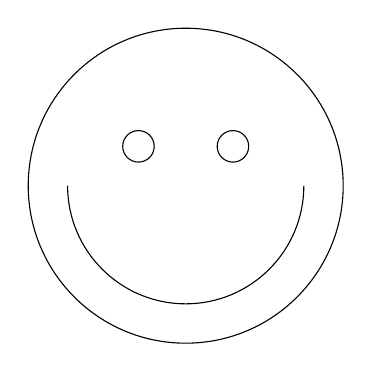
\begin{tikzpicture}
		% Circulo con centro en (0,0), radio de 1
		\draw (0, 0) circle (2);

		% Arco: centro en (0, 0), angulo de 0 a 45 grados, radio de 2
		\draw (1.5, 0) arc (0: -180: 1.5);

		\draw (-0.6, 0.5) circle (0.2); % ojo izquierdo
		\draw (0.6, 0.5) circle (0.2); % ojo derecho
	\end{tikzpicture}
\end{center}
\vspace{0.5cm} % separación vertical

Si quisieras ver las líneas conectadas, puedes eliminar las líneas que llaman a \code{moveTo()}.

\subsubsection{Líneas}

Para dibujar líneas rectas, utilice el método \code{lineTo()}.

\begin{description}
	\listCustom{lineTo(x, y):} Dibuja una línea desde la posición actual de dibujo hasta la posición especificada por \textblue{x} e \textblue{y}.
\end{description}
\vspace{0.5cm} % separación vertical

Este método toma dos argumentos, \textblue{x} e \textblue{y}, que son las coordenadas del punto final de la línea. El punto de partida depende de los trazos anteriores, donde el punto final del trazo anterior es el punto de partida del siguiente, etc. El punto de partida también puede cambiarse utilizando el método \code{moveTo()}.

\newpage % saltar a la siguiente pagina
El ejemplo siguiente dibuja dos triángulos, uno relleno y otro contorneado.

\vspace{0.5cm} % separación vertical
\begin{lstlisting}[language=TypeScript, style=mystyle]
  function draw() {
    const canvas = document.getElementById("canvas");
    if (canvas.getContext) {
      const ctx = canvas.getContext("2d");

      // Triangulo relleno
      ctx.beginPath();
      ctx.moveTo(25, 25);
      ctx.lineTo(105, 25);
      ctx.lineTo(25, 105);
      ctx.fill();

      // Triangulo contorneado
      ctx.beginPath();
      ctx.moveTo(125, 125);
      ctx.lineTo(125, 45);
      ctx.lineTo(45, 125);
      ctx.closePath();
      ctx.stroke();
    }
  }
\end{lstlisting}
\vspace{0.5cm} % separación vertical

Esto comienza llamando a \code{beginPath()} para iniciar un nuevo trazo. A continuación, utilizamos el método \code{moveTo()} para mover el punto de partida a la posición deseada. Debajo de esto, se dibujan dos líneas que forman los dos lados del triángulo.

\vspace{0.5cm} % separación vertical
\begin{center}
	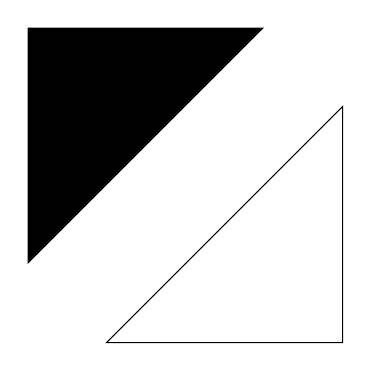
\begin{tikzpicture}
		% Triangulo relleno
		\fill[black] (0,0) -- (3,0) -- (0,-3) -- cycle;
		\draw (4, -1) -- (4, -4) -- (1, -4) -- cycle;
	\end{tikzpicture}
\end{center}
\vspace{0.5cm} % separación vertical

Notará la diferencia entre el triángulo relleno y el trazo. Esto se debe, como se ha mencionado anteriormente, a que las formas se cierran automáticamente cuando se rellena un trazo, pero no cuando se traza. Si omitimos el \code{closePath()} para el triángulo trazo, sólo se habrían dibujado dos líneas, no un triángulo completo.

\newpage % saltar a la siguiente pagina
\subsubsection{Arcos}

Para dibujar arcos o círculos, utilizamos los métodos \code{arc()} o \code{arcTo()}.

\begin{description}
	\listCustom{arc(x, y, radius, startAngle, endAngle, anticlockwise):} Dibuja un arco centrado en la \\ posición \code{(x, y)} con radio \code{r} que comienza en \code{startAngle} y termina en \code{endAngle} yendo en la dirección indicada por \code{counterclockwise} (por defecto en el sentido de las agujas del reloj).

	\listCustom{arcTo(x1, y1, x2, y2, radius):} Dibuja un arco con los puntos de control y el radio dados, conectado al punto anterior por una línea recta.
\end{description}
\vspace{0.5cm} % separación vertical

Veamos con más detalle el método \textblue{arc}, que toma seis parámetros: \textblue{x} e \textblue{y} son las coordenadas del centro del círculo sobre el que se dibujará el arco. El parámetro radio se explica por sí mismo. Los parámetros \code{startAngle} y \code{endAngle} definen los puntos inicial y final del arco en radianes, a lo largo de la curva del círculo. Se miden desde el \lineCode{eje x}. El parámetro \code{counterclockwise} es un valor \lineCode{Booleano} que, cuando es \code{true}, dibuja el arco en sentido contrario a las agujas del reloj; en caso contrario, el arco se dibuja en sentido de las agujas del reloj.

\vspace{0.5cm} % separación vertical
\begin{tcolorbox}
	[colback=red!5!white,colframe=cyan,fonttitle=\bfseries,title={\faLightbulbO\, Nota:}]

	Los ángulos en la función \code{arc()} se miden en radianes, no en grados. Para convertir los grados en radianes puedes utilizar la siguiente expresión de \textjs{JavaScript}:

	\vspace{0.5cm} % separación vertical
	\begin{center}
		\lineCode{ radianes = (Math.PI/180)*grados }
	\end{center}
\end{tcolorbox}
\vspace{0.5cm} % separación vertical

El siguiente ejemplo es un poco más complejo que los que hemos visto anteriormente. Dibuja 12 arcos diferentes, todos con diferentes ángulos y rellenos.

Los dos bucles \lineCode{\textbf{for}} son para recorrer las filas y columnas de arcos. Para cada arco, iniciamos un nuevo trazo llamando a \code{beginPath()}. En el código, cada uno de los parámetros del arco está en una variable para mayor claridad, pero no necesariamente se haría eso en la vida real.

Las coordenadas \textblue{x} e \textblue{y} deberían ser lo suficientemente claras. radius y \code{startAngle} son fijos. \code{endAngle} comienza en 180 grados (medio círculo) en la primera columna y se incrementa en pasos de 90 grados, culminando en un círculo completo en la última columna.

La sentencia para el parámetro \code{clockwise} hace que la primera y tercera fila se dibujen como arcos en el sentido de las agujas del reloj y la segunda y cuarta fila como arcos en sentido contrario. Por último, la sentencia \lineCode{\textbf{if}} hace que la mitad superior tenga arcos trazados y la mitad inferior arcos rellenos.

\vspace{0.5cm} % separación vertical
\begin{tcolorbox}
	[colback=red!5!white,colframe=cyan,fonttitle=\bfseries,title={\faLightbulbO\, Nota:}]

	Este ejemplo requiere un \code{canvas} ligeramente más grande que los otros de esta página:\\
	150 x 200 pixels.
\end{tcolorbox}
\vspace{0.5cm} % separación vertical

\newpage % nueva página
\begin{lstlisting}[language=TypeScript, style=mystyle]
  function draw() {
    const canvas = document.getElementById("canvas");
    if (canvas.getContext) {
      const ctx = canvas.getContext("2d");

      for (let i = 0; i < 4; i++) {
        for (let j = 0; j < 3; j++) {
          ctx.beginPath();
          const x = 25 + j * 50; // Coordenada x
          const y = 25 + i * 50; // Coordenada y
          const radius = 20; // Radio del Arco
          const startAngle = 0; // Punto inicial del Circulo
          const endAngle = Math.PI + (Math.PI * j) / 2; // Punto final del Circulo
          const counterclockwise = i % 2 !== 0; // En el sentido de las agujas del reloj o en sentido contrario

          ctx.arc(x, y, radius, startAngle, endAngle, counterclockwise);

          if (i > 1) {
            ctx.fill();
          } else {
            ctx.stroke();
          }
        }
      }
    }
  }
\end{lstlisting}

El resultado de todo ese código es el siguiente:

\vspace{0.5cm} % separación vertical
\begin{center}
	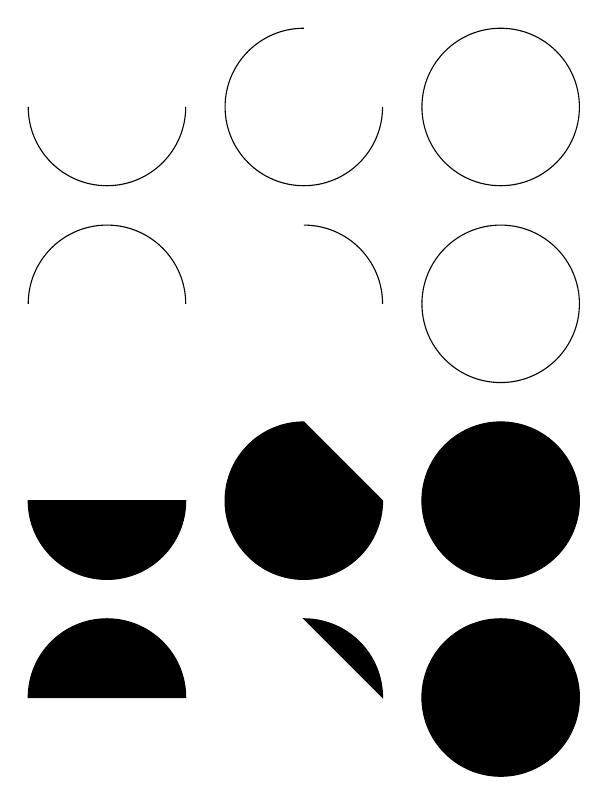
\begin{tikzpicture}
		% arcos y círculos solo con borde
		\draw (0, -1) arc (0:-180:1); % center (0,0); start 0, end -180; radius 1
		\draw (2.5, -1) arc (0:-270:1); % center (2.5, -1); start 0, end -270; radius 1
		\draw (4, -1) circle (1); % center (4, -1); radius 1
		\draw (0, -3.5) arc (0:180:1); % center (0, -3.5); start 0, end 180; radius 1
		\draw (2.5, -3.5) arc (0:90:1); % center (2.5, -3.5); start 0, end 90; radius 1
		\draw (4, -3.5) circle (1); % center (4, -3.5); radius 1

		% arcos y círculos con fill
		\filldraw[fill=black] (0, -6) arc (0:-180:1) -- cycle; % center (0, -6); start 0, end -180; radius 1
		\filldraw[fill=black] (2.5, -6) arc (0:-270:1) -- cycle; % center (2.5, -6); start 0, end -270; radius 1
		\filldraw[fill=black] (4, -6) circle (1) -- cycle; % center (4, -6); radius 1
		\filldraw[fill=black] (0, -8.5) arc (0:180:1) -- cycle; % center (0, -8.5); start 0, end 180; radius 1
		\filldraw[fill=black] (2.5, -8.5) arc (0:90:1) -- cycle; % center (2.5, -8.5); start 0, end 90; radius 1
		\filldraw[fill=black] (4, -8.5) circle (1) -- cycle; % center (4, -8.5); radius 1
	\end{tikzpicture}
\end{center}
